\section{Related Work}\label{sc:works}
\begin{table*}[t!]
\renewcommand{\arraystretch}{0.6}
    \centering
    \footnotesize
\begin{tabular}{l|c|c|c|c|c|c|c|c}
\textbf{Research} & \textbf{Year} & \textbf{Control-plane} & \textbf{Data-plane} & \textbf{Methodology with} & \textbf{Clients} & \textbf{>1 Target} & \textbf{Rate of} & \textbf{\#ASes}\\
 &  & \textbf{} & \textbf{} & \textbf{Divergence} & & \textbf{AS} & \textbf{ROV-ASes} \\\hline \hline
This work & 2022 & \cmark  & Traceroute/Atlas & \cmark & \xmark & \cmark & 27\% & 2.4K\\ \hline
Cloudflare \cite{cloudflare} & 2022 & \xmark & HTTP & \xmark & Volunteers & \xmark & 30\% & 380 \\ \hline
Rodday et al. \cite{rodday2021revisiting} & 2021 & \cmark  & Traceroute/Atlas & \xmark & \xmark & \xmark & 0.6\% & 3.6K\\ \hline 
APNIC \cite{apnic} & 2021 & \cmark & HTTP & \xmark & Ad-network & \xmark & 25\% & 25K \\ \hline
Testart et al. \cite{testart2020filter} & 2020 & RouteViews & \xmark & \xmark & \xmark & \xmark & 11\% & 21 \\ \hline
Hlavacek et al. \cite{hlavacek2018practical} & 2018 & \cmark & Traceroute/Atlas & \xmark & \xmark & \cmark & 0.5\% & 296\\ \hline
Gilad et al. \cite{gilad2017we} & 2017 & \cmark & \xmark & \xmark & \xmark & \xmark & 3\% & 100 \\ %\hline
\end{tabular}
\vspace{-7pt}
\caption{Measurements of ROV: characteristics of our and previous work.}
\vspace{-10pt}
\label{tab:comparison}
\end{table*}
Practical impact of BGP prefix hijacks has been extensively explored \cite{DBLP:conf/uss/Birge-LeeSERM18,DBLP:journals/corr/abs-2004-09063} and real-world hijack incidents \cite{china:telecom,mitm:threat,turkey:hijack,indosat:hijack} confirmed the projected assessment of the research. The awareness to prefix hijacks creates a strong motivation to understand the deployment of RPKI and to obtain insights into the effectiveness of ROV. Previous measurements studied related aspects, such as the prevalence of invalid ROA objects caused by benign misconfigurations \cite{chung2019rpki,DBLP:conf/esorics/HlavacekSW22}, the impact of the Domain Name System on the resilience of RPKI \cite{DBLP:conf/ccs/HlavacekJMSW22} or downgrade attacks against RPKI \cite{usenix-stalloris-21,DBLP:conf/ccs/MirditaSW22}. In this work we explore the effectiveness of ROV. We next put our research in the context of related work on measurements of ROV.

{\bf Effectiveness of ROV.} Previous work provided a theoretical upper bound on the feasibility of hijacks \cite{gilad2017we,hlavacek2020disco}. 
This was done by simulating success of any Internet AS to hijack any prefix assuming a varying fraction of ROV-enforcing ASes. Such simulations do not consider the data-plane paths that actual traffic takes and do not use the real ASes that de facto enforce ROV, but just assume a fraction of ROV enforcement. Therefore the theoretical bound does not reflect a realistic attack surface.
In addition to not reflecting practical factors relevant to success of hijacks, the simulations do not answer questions related to the effectiveness of ROV in blocking propagation of hijacks and to the affected networks. For instance, not all hijacks have equal impact and hijacking a Tier-1 provider also redirects the traffic of all its customers. Our goal is not only to understand if hijacks are feasible, but also to infer which and how many networks are affected by the hijacks and by the ROV filtering. We do this by analyzing the date-plane paths that traffic takes, and the impact of ROV on the Internet graph of networks. We use the observations from our analysis to derive future directions that deployment of ROV should take to reach optimal protection of the Internet. 


{\bf Approaches for measuring ROV.} 
The first global measurement of ROV enforcement was carried out in 2017 \cite{gilad2017we} (listed in Table \ref{tab:comparison}). The study monitored the propagation of invalid BGP announcements in public BGP collectors and found 100 ROV-enforcing ASes. In their experiment, Gilad et al. \cite{gilad2017we} passively monitored ASes that originated valid and invalid BGP announcements, and then collected ASes that were on the paths towards the valid prefix, but not on the paths towards the invalid prefix. Those ASes were classified as ROV-enforcing. However, the measurements had high false positives and false negatives rates since they used invalid BGP announcements of other ASes, which they did not control. This also limited the coverage of the experiment. The methodology of \cite{gilad2017we} was improved with a controlled experiment in the control plane by \cite{hlavacek2018practical}, which monitored propagation of invalid announcements in public collectors and used active probes over RIPE Atlas. The study of \cite{hlavacek2018practical} found 296 ROV-enforcing ASes. A subsequent study in 2020 \cite{testart2020filter} passively analyzed the historical data from RouteViews\footnote{\url{http://www.routeviews.org}} to identify changes in routing behavior, finding 21 ROV-enforcing ASes. Since these measurements were performed using a limited number of collectors (less than 0.01\%) the results were not representative of the entire Internet. Increasing the coverage is imperative for collecting representative data. In 2021 \cite{rodday2021revisiting} did an ROV study with a methodology of \cite{hlavacek2018practical} using 5537 probes in 3694 origin ASes. 

In our work, we combine control and data-plane measurements similarly to \cite{hlavacek2018practical,rodday2021revisiting}. In contrast to \cite{hlavacek2018practical,rodday2021revisiting}, which used an invalid ROA conflicting with a BGP announcement to infer ROV enforcement, we alternate between valid and invalid BGP announcements, which has faster convergence time than changes in ROAs. Alternating between valid and invalid events using two prefixes during data acquisition further allows us to eliminate random routing events, such as events in which an AS uses traffic engineering that complies with the ROA validity, which may be misinterpreted as ROV. This alternation reduces false positives. In addition, the previous method does not scale since it adds a large number of false negatives that lack sufficient evidence for ROV enforcement. We explain the issues with false-positives and false-negatives in previous work when we derive our methodology from previous approaches in Section \ref{sc:method}. In our ROV measurements, we greatly reduce the number of false-negatives and thus provide a more realistic view of real-world ROV enforcement. During data analysis, we apply a path-aware methodology that uses a new metric, divergence points, to reduce false positives. Further, we introduce an AS classification scheme to differentiate ASes that actively enforce ROV from ASes with only passive protection in an upstream ROV. Our approach shows a much higher rate of ROV deployment in the Internet than previously found in \cite{hlavacek2018practical,rodday2021revisiting}, including extensive evidence for enforcement in 9 of the 15 Tier-1 providers. We show that the higher rates of ROV enforcement are related to the improvements in our methodology and the continuous increase of ROV enforcement rate over time.

 
 In 2023, an online service called RoVista\footnote{\url{https://rovista.netsecurelab.org/}} was set up for reporting ROV enforcement. Similarly to \cite{gilad2017we}, RoVista uses an uncontrolled control-plane experiment, utilizing ASes with invalid BGP announcements and probing the reachability to the invalid prefixes from other systems in the Internet. Since they use invalid routes that happen to be announced by other ASes, their coverage is limited; currently, as they point out, only 1\% of prefixes are RPKI invalid. Additionally, they have the same downsides as uncontrolled experiments like \cite{gilad2017we}, which include a high rate of false positives. For instance, ASes might appear to behave like ROV filtering networks because of other (non-ROV) mechanisms. A more significant issue with RoVista is the usage of IPID side channel to identify ASes that follow invalid routes. There are three problems with IPID side channels. First, globally incrementing IPID has been gradually phased out in operating systems. Previous work \cite{pearce2017augur,dai2021smap,DBLP:conf/dsn/ShulmanZ21} showed that very few hosts ($\sim$16\%) had globally incrementing IPID counters and that some hosts with globally incrementing counters set their values to 0 when packets are too small to be fragmented. RoVista additionally requires that multiple ASes have at least ten hosts with globally incrementing IPID. The authors do not provide the methodology and measurement details on how many ASes have at least ten hosts with globally incrementing IPID counters. Since previous work showed that the number of hosts with global incrementing IPID is small and is further shrinking, the approach has limited scalability. 

 Second, measurements of IPID incur a lot of noise due to communication from other hosts, failures, and traffic fluctuations. Simple applications that use IPID, such as indirect measurements of idle port scans with NMap, exhibit high failure rates in dynamic Internet environments with over 10\% failures in scans of even completely idle hosts. These measurements were slightly improved with anti-noise techniques used by \cite{zhang2018onis}. Using the IPID side channel to measure ROV enforcement appears to be much more challenging than just checking if a port is open. In particular, there is a large time interval between the probing of the IPID value and the time that the BGP announcements converge and the routes are updated. The lack of visibility into the exact time when the route change is accepted makes it impossible to approximate the probe time of the IPID value. This is expected to introduce an immense amount of noise into the measurements, producing many false negatives and positives, making it impossible to derive a conclusion on ROV enforcement. The authors do not explain how they deal with that noise. Finally, the traffic volume to the ASes that announce the invalid prefixes would become prohibitive in the presented methodology as all the tested networks are required to send traffic to these ASes from ten of their hosts, resulting in regular traffic from 280.000 hosts. In total, they send traffic from these hosts to 47 ASes that announce invalid prefixes. The lack of methodology details of the measurements done by RoVista makes it impossible to compare our study to theirs and to understand the correctness or effectiveness of their approach. 

A completely different approach was taken by the Cloudflare project \footnote{https://isbgpsafeyet.com/}, which is a community-driven effort to summarize ROV implementation of large providers. The project provides a webpage to test ROV enforcement of providers by probing the reaction of the client to a valid and invalid announcement. If a client can reach the valid announcement and not the invalid one, they conclude that the provider of the client enforces ROV. The user can then contribute to the project over a GitHub page and update the status of its provider in the dataset. Our measurements show that while this approach may be sensible for a rough overview of large ROV-enforcing networks, it does not scale to an accurate representation of ROV enforcement in the Internet. 
In contrast to previously described approaches, Cloudflare requires coordination and support of volunteers to measure ROV enforcement in the networks of the users, which proves problematic.
First, the dataset is small, with only 380 ASes. Second, smaller ASes with fewer clients are less likely to have a user that contributes, and thus the dataset is biased towards the largest providers. 
We also find false positives in the results. Since the measurement methodology relies on two announcements picked up by a single vantage point, it leads to errors in cases where the ROV in an upstream provider filters the invalid announcement. The provider of the user is mistakenly classified as ROV-enforcing. 
This approach thus not only limits the applicability of ROV measurements in the global Internet but also introduces a bias to the results. We evaluated the Cloudflare dataset and identified differences and errors in the classification, which we discuss in Section \ref{subsec:vali}.


\begin{figure}[t!]
    \centering
    \scalebox{0.8}{
    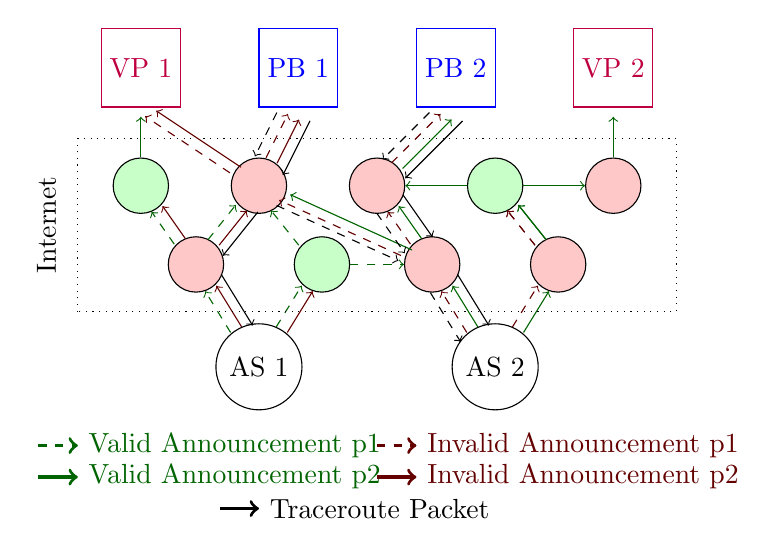
\begin{tikzpicture}
       \tikzset{vertex/.style = {shape=circle,draw,minimum size=2em}}
       \tikzset{vertex2/.style = {shape=circle,draw,minimum size=2.5em}}
       \tikzset{edge1l/.style = {dashed, ->, transform canvas={xshift=-2pt, yshift=-1pt}}}
       \tikzset{edge1r/.style = {dashed, ->, transform canvas={xshift=-2pt, yshift=1pt}}}
       \tikzset{edge2l/.style = { ->, transform canvas={xshift=2pt, yshift=1pt}}}
       \tikzset{edge2r/.style = { ->, transform canvas={xshift=2pt, yshift=-1pt}}}
       
       \tikzset{edge3l/.style = {->, transform canvas={xshift=6pt, yshift=-1.5pt}, shorten >=-0.15cm}}
        \tikzset{edge3r/.style = {->, transform canvas={xshift=6pt, yshift=1.5pt}, shorten <=-0.15cm}}

       \tikzset{edge4l/.style = {->, transform canvas={xshift=-6pt, yshift=1.5pt}}}
       \tikzset{edge4r/.style = {->, transform canvas={xshift=-6pt, yshift=-1.5pt}, shorten >=-0.12cm}}
       
       \definecolor{node_red}{RGB}{255, 200, 200}
        \definecolor{node_green}{RGB}{200, 255, 200}
        \definecolor{c_green}{RGB}{0, 100, 0}
        \definecolor{c_red}{RGB}{100,0 , 0}

        \node[vertex] (a) at (0.5, 1.2) {AS 1};
        \node[vertex] (b) at (3.5, 1.2) {AS 2};
        
        \node[vertex, fill=node_red] (c) at (-0.3, 2.5) {};
        \node[vertex, fill=node_green] (d) at (1.3, 2.5) {};
        \node[vertex, fill=node_red] (e) at (2.7, 2.5) {};
        \node[vertex, fill=node_red] (f) at (4.3, 2.5) {};
        
        \node[vertex, fill=node_green] (g) at (-1, 3.5) {};
        \node[vertex, fill=node_red] (h) at (0.5, 3.5) {};
        \node[vertex, fill=node_red] (i) at (2, 3.5) {};
        \node[vertex, fill=node_green] (j) at (3.5, 3.5) {};
  
        \node[vertex, fill=node_red] (k) at (5, 3.5) {};
        
        \draw[purple] (-1.5,4.5) rectangle (-0.5,5.5) node[pos=.5] {VP 1};
        \draw[blue] (0.5,4.5) rectangle (1.5,5.5) node[pos=.5] {PB 1};
        \draw[blue] (2.5,4.5) rectangle (3.5,5.5) node[pos=.5] {PB 2};
        \draw[purple] (4.5,4.5) rectangle (5.5,5.5) node[pos=.5] {VP 2};
        
        \node (l) at (-1, 4.5){};
        \node (m) at (1, 4.5){};
        \node (n) at (3, 4.5){};
        \node (o) at (5, 4.5){};
        
        
        
        \draw[edge1l, c_green] (a) to (c);
        \draw[edge2l, c_red] (a) to (c);
        \draw[edge1r, c_green] (a) to (d);
        \draw[edge2r, c_red] (a) to (d);
        
        \draw[edge1l, c_red] (b) to (e);
        \draw[edge2l, c_green] (b) to (e);
        \draw[edge1r, c_red] (b) to (f);
        \draw[edge2r, c_green] (b) to (f);
        
        \draw[edge1l, c_green] (c) to (g);
        \draw[edge2l,  c_red] (c) to (g);
        
        \draw[edge1r, c_green] (c) to (h);
        \draw[edge2r,  c_red] (c) to (h);
        
        \draw[edge1l, c_green] (d) to (h);
        
        \draw[edge1l, c_red] (e) to (h);
        \draw[edge2l, c_green] (e) to (h);
        
        \draw[edge1l, c_red] (e) to (i);
        \draw[edge2l, c_green] (e) to (i);
        
        \draw[edge1l, c_red] (f) to (j);
        \draw[edge2l, c_green] (f) to (j);
        
        \draw[->, c_green] (j) to (k);

        \draw[->, c_green] (j) to (i);

        \draw[dashed, ->, c_green] (d) to (e);
        
        
        \node[rotate=90] at (-2.2, 3.0 ){Internet};
        \draw[dotted] (-1.8, 1.9) rectangle (5.8, 4.1);
        
        \draw[edge1l, c_red] (f) to (j);
        \draw[edge2l, c_green] (f) to (j);
        
        \draw[->, c_green] (g) to (l);
        
        \draw[edge1l, c_red] (h) to (l);
        \draw[edge2l, c_red] (h) to (l);
        
        \draw[edge1r, c_red] (h) to (m);
        \draw[edge2r, c_red] (h) to (m);
        
        \draw[edge1r, c_red] (i) to (n);
        \draw[edge2r, c_green] (i) to (n);
        
        \draw[->, c_green] (k) to (o);
        
        \draw[edge3l] (m) to (h);
        \draw[edge3l] (h) to (c);
        \draw[edge3r] (c) to (a);

        \draw[edge4l, dashed] (m) to (h);
        \draw[edge4r, dashed, shorten <=0.12cm] (h) to (e);
        \draw[edge4r, dashed] (e) to (b);
        
        
        \draw[edge3l] (n) to (i);
        \draw[edge3r] (i) to (e);
        \draw[edge3r] (e) to (b);
        
        \draw[edge4l, dashed, shorten >=0.04cm] (n) to (i);
        
        \draw[edge4r, dashed] (i) to (e);

        \draw[->, very thick, c_green, dashed] (-2.3,0.2) --++ (0.5,0) node[right]{Valid Announcement p1};
        \draw[->, very thick, c_red, dashed] (2.0,0.2) --++ (0.5,0) node[right]{Invalid Announcement p1};
        
        \draw[->, very thick, c_green] (-2.3,-0.2) --++ (0.5,0) node[right]{Valid Announcement p2};
        \draw[->, very thick, c_red] (2.0,-0.2) --++ (0.5,0) node[right]{Invalid Announcement p2};
        
        \draw[->, very thick] (-0,-0.6) --++ (0.5,0) node[right]{Traceroute Packet};
            \end{tikzpicture}
    }
    \caption[Overview RPKI Process]%
    {Measurement setup with AS 1 and AS 2 with prefixes p1 and p2. Vantage Points 1 and 2 collect received announcements, the probes PB1 and PB2 use received paths to send out Traceroutes to both prefixes.}
    \label{fig:setup}
    \vspace{-10pt}
    
\end{figure} 

Similarly to Cloudflare, the Asia-Pacific Network Information Centre (APNIC) runs an experiment to test ROV deployment over the reachability of destinations with varying ROV validity \footnote{\url{https://stats.labs.apnic.net/rpki}}. 
The measurement probes how many users in a specific AS can reach an invalid prefix to draw conclusions on the ROV enforcement status of that user’s AS. 
The APNIC measurement improves over the Cloudflare project in two keys aspect. First, they do not rely on users to visit the website and then manually contribute the enforcement status of their provider over a Github page. Instead, they automatically execute the measurement on client systems. Second, they use anycast to inject their route from a large amount of routers instead of two points used by Cloudflare. This significantly reduces the rate of false-positives. ROV enforcement in intermediate systems is less likely to affect the measurement if the route is propagated over many different paths to a target. In Section \ref{sc:rov} we use APNIC's dataset to validate our measurements and provide insights into the limitations and challenges inherent in comparing different ROV measurement methodologies. 